\documentclass[a4paper, 14pt, titlepage, fleqn]{extarticle}
\usepackage[russian]{babel}
\usepackage{amsmath}
\usepackage{csquotes}
\usepackage{graphicx}
\usepackage[justification=centering]{caption}
\usepackage{float}
\usepackage{mathtools}

\DeclareMathOperator\artanh{artanh}
\DeclareMathOperator\sech{sech}
\DeclareMathOperator\Si{Si}
\DeclareMathOperator\Ei{Ei}
\DeclareMathOperator\li{li}

\author {
	Группа Б9120-01.03.02миопд\\
	Агличеев Александр
}
\title {
	Отчёт по лабораторной работе №2
}
\date {
	\today
}


\begin{document}
	\maketitle
	\tableofcontents
	\pagebreak	

	\section*{Введение}
	\addcontentsline{toc}{section}{Введение}
		В данной лабораторной работе мне нужно найти общее решение и построить векторное после с помощью программ компьютерной математики, решить задачу Коши и проверить решение задачи Коши.
	
	\pagebreak
	\section*{Задание 1}
	\addcontentsline{toc}{section}{Задание 1}
		\subsection*{Постановка задачи}
		\addcontentsline{toc}{subsection}{Постановка задачи}
			\noindent Для следующих дифференциальных уравнений определить тип, найти общее
			решение и построить векторное поле с помощью программ компьютерной математики:
		\begin{enumerate}
			 \item \(\sinh{x} \cdot \cosh{x} + y - 1 = ( \sinh{y} \cdot \cosh{y}) \cdot y'\)
			 \item \(xy' - 4 \tan{y} = 2x^2 \cdot \cos{x^2} \cdot \sec{y} \)
			 \item \(y' \sin{x} - y \cot{x} = \cot{x} \cdot \sin{x} \)
			 \item \( \sec^2{xy} \cdot \tan{xy} \cdot \big(xy' + y\big) + \sech^2{x} - y' \cos{y} = 1 \)
			 \item \( y' \cdot \cos^2{x} = \sec{y} \cdot \ln{\sin{y}} \)
		\end{enumerate}
		\subsection*{Решение}
		\addcontentsline{toc}{subsection}{Решение}
			\noindent Поиск решения и построение векторного поля будет проводиться в системе компьютерной математики Wolfram Mathematica.
			\begin{enumerate}
				\item \(  \sinh{x} \cdot \cosh{x} + y - 1 = ( \sinh{y} \cdot \cosh{y} - x - 1) \cdot y'\)

					\textit{Тип уравнения:} Уравнение в полных дифференциалах
		
					\textit{Ответ:} \( \sinh^2{y} - \sinh^2{x} + 2x - 2xy - 2y = C \)
					
					\begin{figure}[H]
					    	\centering
					    	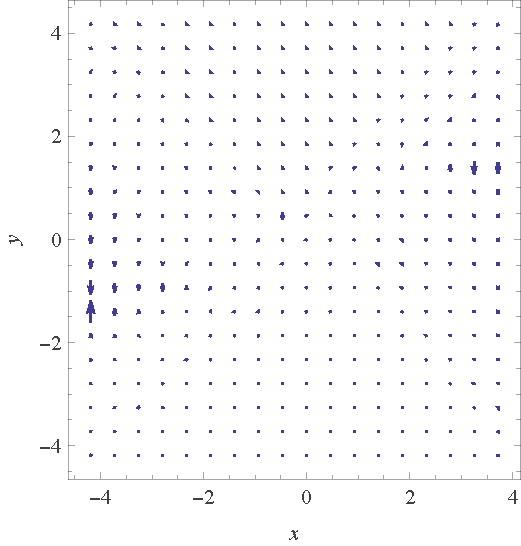
\includegraphics[width = .5\linewidth]{1.pdf}
					   	 \caption[.] {Векторное поле \\ \(\sinh{x} \cdot \cosh{x} + y - 1 = ( \sinh{y} \cdot \cosh{y}) \cdot y'\)}
  					\end{figure}

				\item \( xy' - 4 \tan{y} = 2x^2 \cdot \cos{x^2} \cdot \sec{y}\)
		
					\textit{Тип уравнения:} Линейное неоднородное неприведенное уравнение первого порядка с постоянными коэффициентами относительно переменной \( u = \sin{y} \)
		
					\textit{Ответ:} \( \sin{y} = Cx^4 + x^2 \cdot \big(x^2\Si{(x^2)} + \cos{x^2}\big) \)

					\begin{figure}[H]
					    	\centering
					    	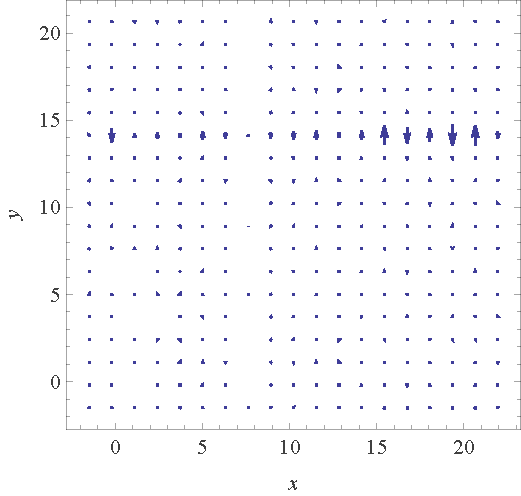
\includegraphics[width = .5\linewidth]{2.pdf}
						\caption[.] {Векторное поле \\  \( xy' - 4 \tan{y} = 2x^2 \cdot \cos{x^2} \cdot \sec{y}\)}
  					\end{figure}
				\item \( y' \sin{x} - y \cot{x} = \cot{x} \cdot \sin{x} \)
		
					\textit{Тип уравнения:} Линейное неоднородное неприведенное уравнение первого порядка с постоянными коэффициентами относильное переменной \( y \)
		
					\textit{Ответ:} \( y =e^{-\csc{x}} \cdot \big(C -\Ei{(\csc{x})}\big) \)

					\begin{figure}[H]
					    	\centering
					    	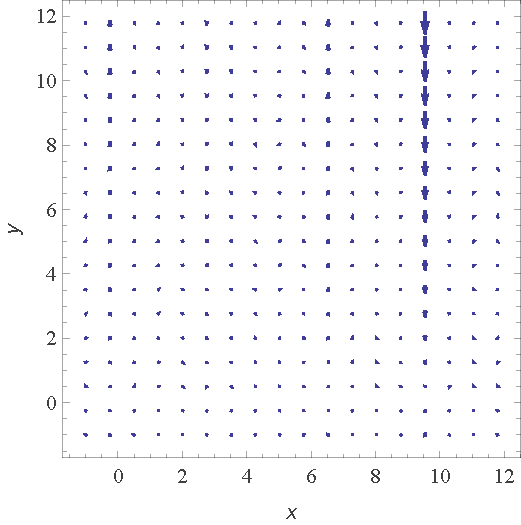
\includegraphics[width = .5\linewidth]{3.pdf}
						\caption[.] {Векторное поле \\  \( y' \sin{x} - y \cot{x} = \cot{x} \cdot \sin{x} \)}
  					\end{figure}
		
				\item \( \sec^2{xy} \cdot \tan{xy} \cdot \big(xy' + y\big) + \sech^2{x} - y' \cos{y} = 1 \)
		
					\textit{Тип уравнения:} Уравнение в полных дифференциалах
	
					\textit{Ответ:} \( \tg^2{xy} + 2\tanh{x} - 2\sinh{y} - 2x = C \)
					
					\begin{figure}[H]
					   	\centering
					    	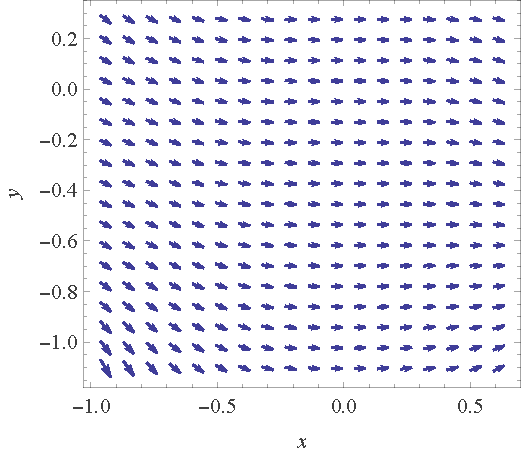
\includegraphics[width = .5\linewidth]{4.pdf}
						\caption[.] {Векторное поле \\  \( \sec^2{xy} \cdot \tan{xy} \cdot \big(xy' + y\big) + \sech^2{x} - y' \cos{y} = 1 \)}
  					\end{figure}
				
				\item \( y' \cdot \cos^2{x} = \sec{y} \cdot \ln{\sin{y}} \)
		
					\textit{Тип уравнения:} Уравнение с разделяющимся переменными
	
					\textit{Ответ:} \( \li{(\sin{y})} - \tan{x} = C \)

					\begin{figure}[H]
					    	\centering
					    	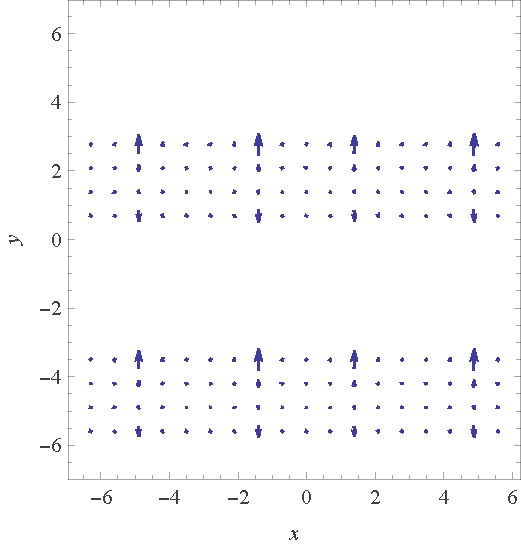
\includegraphics[width = .5\linewidth]{5.pdf}
						\caption[.] {Векторное поле \\  \( y' \cdot \cos^2{x} = \sec{y} \cdot \ln{\sin{y}} \)}
  					\end{figure}
			\end{enumerate}

	\pagebreak
	\section*{Задание 2}
	\addcontentsline{toc}{section}{Задание 2}
		\subsection*{Постановка задачи}
		\addcontentsline{toc}{subsection}{Постановка задачи}
			\noindent Решить задачу Коши, построить график решения:
			\begin{enumerate}
				\item \(y' = e^{-x^2} - 2xy; \quad y(0) = 1\)
				\item \((\cos{x} - \sin{x} \cdot \tan{y}) \cdot y' = \sin{x} + (\cos{x} + \sin{x})\tan{y} - \cos{x};\) 

					\(y(0) = \dfrac{\pi}{2}\)
			\end{enumerate}
		\subsection*{Решение}
		\addcontentsline{toc}{subsection}{Решение}
			\begin{enumerate}
				\item \(\bigg\{ \begin{matrix*}[l] y' = e^{-x^2} - 2xy; \\  y(0) = 1; \end{matrix*}\)

					\textit{Тип уравнения:} Линейное уравнение первого порядка относительно переменной \(y\)					

					\textit{Общее решение:} \( y = e^{-x^2}(C+x) \)
	
					\textit{Задача Коши:} \( y = e^{-x^2}(1+x) \)

					\begin{figure}[H]
					   	\centering
					    	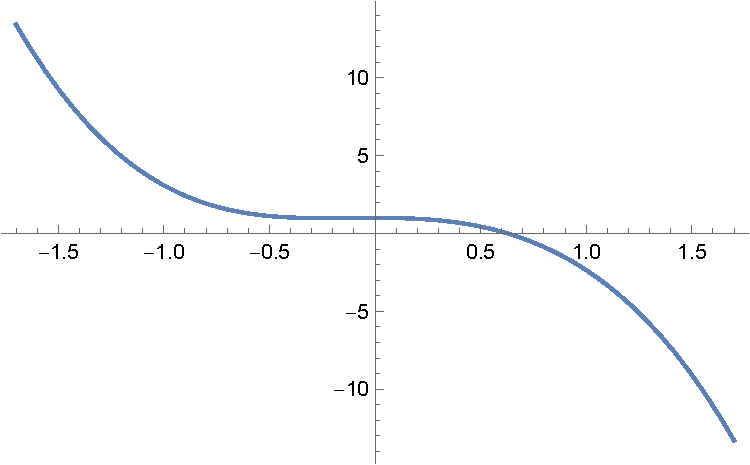
\includegraphics[width = .5\linewidth]{2.1.pdf}
						\caption[.] {График \( y = e^{-x^2}(1+x) \)}
  					\end{figure}
					\begin{figure}[H]
					   	\centering
					    	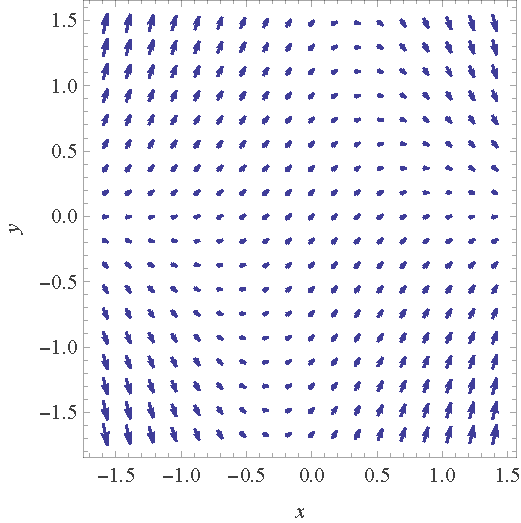
\includegraphics[width = .5\linewidth]{2.1vf.pdf}
						\caption[.] {Векторное поле \( y' = e^{-x^2} - 2xy \)}
  					\end{figure}
				
				\item \(\Bigg\{ \begin{matrix*}[l] (\cos{x} - \sin{x} \cdot \tan{y}) \cdot y' = \sin{x} + (\cos{x} + \sin{x})\tan{y} - \cos{x}; \\ y(0) = \dfrac{\pi}{2}; \end{matrix*}\)

					\textit{Тип уравнения:} Однородное уравнение

					\textit{Общее решение:} \( \sin{(x + y)} = Ce^x \)
	
					\textit{Задача Коши:} \( \sin{(x + y)} = e^x \)

					\begin{figure}[H]
					    	\centering
					    	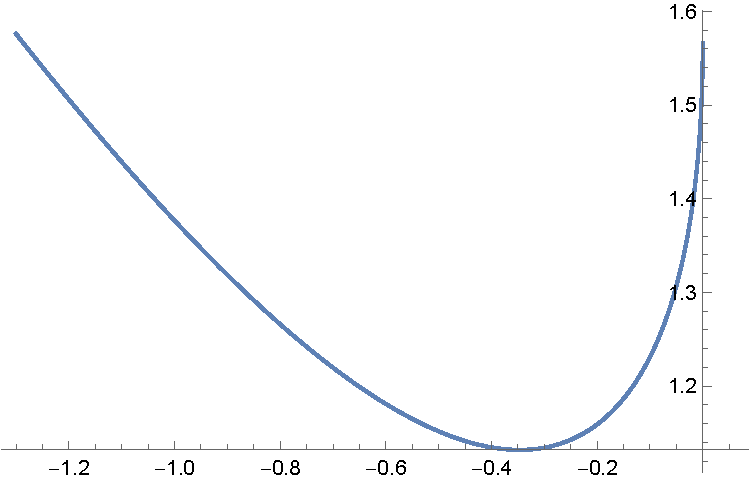
\includegraphics[width = .5\linewidth]{2.2.pdf}
						\caption[.] {График \(\sin{(x + y)} = e^x \)}
  					\end{figure}

					\begin{figure}[H]
					    	\centering
					    	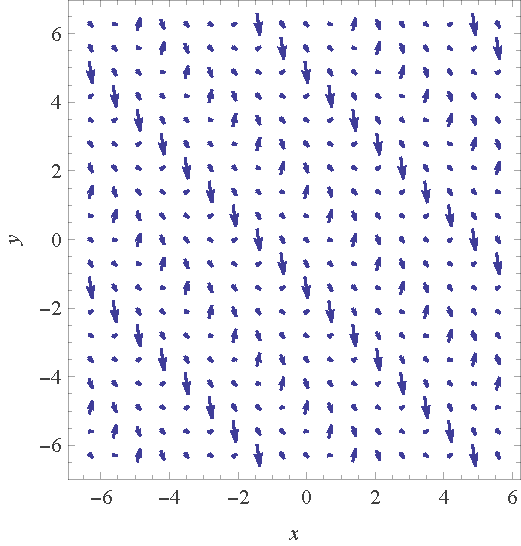
\includegraphics[width = .5\linewidth]{2.2vf.pdf}
						\caption[.] {Векторное поле \\ \( (\cos{x} - \sin{x} \cdot \tan{y}) \cdot y' = \sin{x} + (\cos{x} + \sin{x})\tan{y} - \cos{x} \)}
  					\end{figure}
			\end{enumerate}

	\pagebreak
	\section*{Задание 3}
	\addcontentsline{toc}{section}{Задание 3}
		\subsection*{Постановка задачи}
		\addcontentsline{toc}{subsection}{Постановка задачи}
			\noindent Проверить, является ли, представленная неявная функция решением следующей задачи Коши:
			\[2xy = 2\sin{(x+y)}y' - y\sqrt{1-y^2-x^2}\big(1+y'\big) , y\bigg(\dfrac{\pi}{2}\bigg) = -\dfrac{\pi}{2}; \sin{(x+y)} = y^2-x^2 \]
		\subsection*{Решение}
		\addcontentsline{toc}{subsection}{Решение}
			Проверим начальное условие \( y\bigg(\dfrac{\pi}{2}\bigg) = -\dfrac{\pi}{2} \):
			\begin{align*}
				\sin{\bigg(\dfrac{\pi}{2} - \dfrac{\pi}{2}\bigg)}&= \bigg(\dfrac{\pi}{2}\bigg)^2 - \bigg(\dfrac{\pi}{2}\bigg)^2 \\
				\sin{0}&= 0 \\
				0 &= 0
			\end{align*}
			\noindent Начальное условие выполняется
			\[y' = \dfrac{2x+\cos{(x+y)}}{2y-\cos{(x+y)}}\]

			\noindent Подставим в уравнение и проверим получится ли верное равенство:
			\[2xy = 2\sin{(x+y)} \cdot \bigg ( \dfrac{2x+\cos{(x+y)}}{2y-\cos{(x+y)}} \bigg) - y\sqrt{1-y^2-x^2}\bigg (1+ \dfrac{2x+\cos{(x+y)}}{2y-\cos{(x+y)}} \bigg) \]
			Неявная функция \(  \sin{(x+y)} = y^2-x^2 \) не является решением задачи Коши.

	\section*{Заключение}
	\addcontentsline{toc}{section}{Заключение}
		\noindent Я решил задачи Коши, проверил задачу Коши и c помощью Wolfram Mathematica решил 5 дифференциальных уравнений. Оформлял отчёт по работе  в \textquote{TeX Live}.

\end{document}	